%%%%%%%%%%%%%%%%%%%%%%%%%%%%%%%%%%%%%%%%%%%%%%%%%%%%%%%%%%%%%%%%%
\newpage
\section[Vektorräume (Wdh. Mathe 1)]{Vektorräume, Unterräume und ein Haufen Definitionen (Basen, lineare Unabhängigkeit, Erzeugnis)}
\Einleitung{\red{Achtung, die ersten Kapitel sind eine Aufarbeitung der Themen aus Mathe 1.}
Wir wenden uns zu Beginn einer wichtigen mathematischen Struktur, den Vektorräumen, zu.\\
Viele Objekte, die wir aus der Physik kennen - z. B. Kräfte oder Wellen - zeigen ein Verhalten, das genau dieser Struktur entspricht. Um ordentlich damit umgehen zu können, definieren wir uns ein Netz an Begriffen, um Vektoren und Relationen zwischen Vektoren näher zu klassifizieren.\\
Gerade im Hinblick auf das zweite (und alle weiteren) Semester ist es enorm wichtig, dass ihr diese Begriffe möglichst schnell verinnerlicht.}
\subsection{Vektorräume}\label{ssec:Vektorraum}
Wenn euch von nun an jemand fragt, was ein Vektorraum ist, sollte euch die Definition sofort einfallen:
\begin{Def}
{Vektorraum}
Ein \red{Vektorraum über $\mathbb{K}$}\footnote{$\mathbb{K}$ ist einfach der Körper (wie z. B. $\mathbb{R}$), aus dem die Skalare für die Multiplikation kommen.} ist eine \underline{Menge} $V$ zusammen mit der \red{vektoriellen Addition} und der \red{skalaren Multiplikation} bzgl. von $\mathbb{K}$.\\
\begin{tabular}{l|l|l}
    \textbf{Name} &\textbf{ Definition }&\textbf{ Erklärung} \\
    \hline
    Addition: & $V\times V\to V:\, (v,w)\mapsto v+w$ &\parbox[t]{5cm}{\blue{Die Summe zweier Vektoren ist wieder ein Vektor.}} \\
    Skalare Multiplikation: & $\mathbb{K}\times V\to V:\,(\lambda, v)\mapsto \lambda \cdot v$ & \parbox[t]{5cm}{\blue{Wir können Vektoren skalieren und erhalten dadurch wieder Vektoren.}}
\end{tabular}
Wie wir später sehen werden, nennt man die Kombination aus Addition und Multiplikation verschiedener Vektoren \red{Linearkombination}.
\end{Def}
Addition und Multiplikation müssen dabei bestimmte Eigenschaften erfüllen, damit wir wie gewohnt rechnen können:\\
$(V,+)$ muss eine \underline{kommutative Gruppe} sein.
\begin{Def}
{Kommutative Gruppe}
Für eine kommutative Gruppe $(V,+)$ gelten die folgenden Relationen für alle $v,w,u\in V$:
\begin{enumerate}
    \item \textbf{Kommutativgesetz}:\\
    $v+w=w+v$
    \item \textbf{Assoziativgesetz}:\\
    (u+v)+w=u+(v+w)
    \item \textbf{Nullelement}:\\
    Es existiert $0\in V$, sodass $v+0=v$ gilt.
    \item \textbf{Additives Inverses}:\\
    Für alle $v$ existiert $-v$, sodass $v+(-v)=0$.
\end{enumerate}
Nullelement und additive Inverse sind eindeutig.
\end{Def}
Die skalare Multiplikation muss hingegen folgende Relationen\footnote{Die ihr als Assoziativgesetz, Neutrales Element und Distributivgesetze kennt} erfüllen:
\begin{align*}
    (\lambda\mu)\cdot v&=\lambda(\mu\cdot v)\\
    1\cdot v&= v\\
    (\lambda+\mu)\cdot v&=\lambda \cdot v+\mu \cdot v\\
    \lambda\cdot(v+w)&=\lambda \cdot v+\lambda \cdot w.
\end{align*}
\begin{Beispiel}
{Funktionen bilden einen Vektorraum (2/2)}
Wir können Funktionen $f\in \Abb(X,\mathbb{K})$\footnote{Mit $\Abb(X,\mathbb{K})$ meinen wir Abbildungen von der Menge $X$ in den Körper $\mathbb{K}$.} als Vektoren auffassen bzw. $\Abb(X,\mathbb{K})$ als Vektorraum über $\mathbb{K}$:
\begin{eqnarray*}
+:&&\Abb(X,\mathbb{K})\times \Abb(X,\mathbb{K})\to \Abb(X,\mathbb{K}):\,(f+g)(x)=f(x)+g(x)\quad (x\in X)\\
\cdot:&&\mathbb{K}\times \Abb(X,\mathbb{K})\to \Abb(X,\mathbb{K}):\,(\lambda f)(x)=\lambda\cdot f(x)\quad (\lambda\in\mathbb{K}).
\end{eqnarray*}
\end{Beispiel}
\begin{Beispiel}{Ein kartesischer Raum (2/2)}
Der $\mathbb{R}^3=\{(x,y,z)\furdas x,y,z\in\mathbb{R}\}$ als Spezialfall des kartesischen Raumes (Folie 319 im Mathe-1-Skript) ist mit
\begin{eqnarray*}
+:&&\mathbb{R}^3\times\mathbb{R}^3\to\mathbb{R}^3, \Matrix{x\\y\\z}+\Matrix{a\\b\\c}=\Matrix{x+a\\y+b\\z+c}\text{ und }\\
\cdot:&&\mathbb{R}\times\mathbb{R}^3\to\mathbb{R}^3,\,\lambda\Matrix{x\\y\\z}=\Matrix{\lambda x\\\lambda y\\\lambda z}
\end{eqnarray*}
ein Vektorraum.\\
Als Notation für Vektoren $v\in\mathbb{R}^3$ nutzen wir in diesen Notizen Spaltenvektoren.
\end{Beispiel}
\subsubsection{Untervektorräume}
Für viele Anwendungen benötigen wir nur Teilmengen eines Vektorraums $V$ (anschaulich z. B. eine Ebene im $\mathbb{R}^3$).\\
Diese Teilmenge $U$ erbt automatisch die Addition (A) und Multiplikation (M) des Vektorraumes, jedoch wird zusätzlich die \underline{Abgeschlossenheit} gefordert, d. h. dass wir durch (A) und (M) (also Linearkombinationen von Vektoren aus $U$) nicht plötzlich außerhalb von $U$ landen dürfen.\\
Zudem interessieren uns leere Mengen nicht wirklich, weshalb diese per Definition keine Untervektorräume sind.
\begin{Def}
{Untervektorräume}
Ein \red{Unterraum}\footnote{oder \red{Untervektorraum}} $U$ eines Vektorraumes $V$ über $\mathbb{K}$ muss also folgende Eigenschaften erfüllen:
\begin{enumerate}
    \item \textbf{Teilmenge}:\\
    $U\subseteq V$, \blue{$U$ ist eine Teilmenge von $V$.}
    \item \textbf{Nicht leer}:\footnote{Da freue ich mich bei meinem Kühlschrank auch immer.}\\
    $U\neq\emptyset$, \blue{$U$ ist nicht die leere Menge.}
    \item \textbf{Additive Abgeschlossenheit}:\\
    $v+w\in U\,\forall v,w\in U$, \blue{$U$ ist abgeschlossen bzgl. der vektoriellen Addition.}
    \item \textbf{Multiplikative Abgeschlossenheit}:\\
    $\lambda \cdot v\in U\,\forall \lambda\in\mathbb{K}, v\in U$, \blue{$U$ ist abgeschlossen bzgl. der skalaren Multiplikation.}
\end{enumerate}
\end{Def}

\begin{Satz}
{Vorgehensweise}{Untervektorraum zeigen/Widerlegen}
Wenn ihr also zeigen wollt, dass etwas ein Unterraum ist, müsst ihr für 2) irgendein Element finden - am einfachsten ist häufig der Nullvektor - und anschließend 3) und 4) allgemein zeigen.\\
Zum Widerlegen nutzt ihr einfach 3) oder 4) mit konkreten Elementen.
\end{Satz}
\begin{Beispiel}
{Polynome bilden einen Untervektorraum (1/4)}
\Zz{Polynome von Grad ${\leq n}$ mit Koeffizienten aus $\mathbb{K}$ (im folgenden bezeichnet als $\mathbb{K}[x]_{\leq n}$) der Form
\begin{equation*}
    P:\mathbb{K}\to\mathbb{K},\,x\mapsto P(x)=a_0+a_1x+a_2x^2+...=\sum_{k=0}^na_kx^k
\end{equation*}
bilden einen Untervektorraum der Funktionen von $\mathbb{K}\to\mathbb{K}$ ($\Abb(\mathbb{K},\mathbb{K}$).}
\Zb{(Auch wenn das natürlich kein vollständiger Beweis ist, betrachten wir $\mathbb{K}=\mathbb{R}$, also $\mathbb{R}[x]_{\leq n}\subseteq\Abb(\mathbb{R},\mathbb{R})$.)
\begin{enumerate}\setcounter{enumi}{1}
    \item $\mathbb{R}[x]_{\leq n}$ ist nicht leer, denn $P:\mathbb{R}\to\mathbb{R},\, P(x)=0$ ist ein Polynom ($P\in\mathbb{R}[x]_{\leq n}$).
    \item Seien $P(x):=\sum_{k=0}^na_kx^k$ und $Q(x):=\sum_{k=0}^nb_kx^k\in\mathbb{R}[x]_{\leq n}$. Dann ist
    \begin{equation*}
        P(x)+Q(x)=\sum_{k=0}^na_kx^k+\sum_{k=0}^nb_kx^k=\sum_{k=0}^n(a_k+b_k)x^k=:\sum_{k=0}^nc_kx^k\in \mathbb{R}[x]_{\leq n}.\,\checkmark
    \end{equation*}
    \item Sei zudem $\lambda\in\mathbb{R}$, so gilt
    \begin{equation*}
        \lambda\cdot P(x)=\lambda\sum_{k=0}^na_kx^k=\sum_{k=0}^n\lambda a_kx^k=:\sum_{k=0}^nd_kx^k\in \mathbb{R}[x]_{\leq n}.\,\checkmark
    \end{equation*}
\end{enumerate}}\\
Anmerkung: Nur die Polynome von Grad $n$ (d. h. Polynome der Form $f(x)=\sum_{k=0}^na_kx^k$ mit $a_n\neq0$) bilden KEINEN Untervektorraum, da durch Linearkombination zweier solcher Polynome die Nullfunktion erzeugt werden kann (z. B. $g(x)=f(x)-f(x)=0$ \Lightning), die ja kein Polynom von Grad $n$ mehr ist.
\end{Beispiel}
\begin{Beispiel}
{Die Gerade als Unterraum mit einem Vektor (2/4)}
\begin{tabular}{c l}
\parbox[b]{10cm}{
\Zz{Die Gerade $\mathbb{R}v=\{\mu v\furdas\mu\in\mathbb{R}\}\subseteq\mathbb{R}^2$ ist $\forall v\in\mathbb{R}^2$ der kleinste Unterraum, der $v$ enthält.}
} & 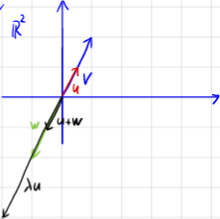
\includegraphics[width=.2\textwidth]{Dateien/00/11GeradeUnterraum.PNG}
\end{tabular}\\
\Zb{Wir zeigen, dass es ein Unterraum ist:\\
Fallunterscheidung: Sei $v=\Vec{0}$, so ist $\mathbb{R}v=\{0\}\subseteq \mathbb{R}^2$ offensichtlich ein Unterraum, der die Eigenschaften erfüllt.\\
Für $v\neq0$: Es seien $u, v\in\mathbb{R}v$ und $\lambda\in\mathbb{R}$
\begin{enumerate}\setcounter{enumi}{1}
    \item $v=1\cdot v$ ist ein Element aus $\mathbb{R}v$, d. h. $\mathbb{R}v$ ist nicht leer.
    \item Es gilt $u+v=\mu_1 v+\mu_2 v=(\mu_1+\mu_2)v=:s\in\mathbb{R}v.\,\checkmark$
    \item Es gilt $\lambda u=\lambda\mu_1 v=(\lambda\mu_1)v=:t\in\mathbb{R}v.\,\checkmark$
\end{enumerate}}
\end{Beispiel}
\begin{Beispiel}
{Affine Geraden sind keine Unterräume (3/4)}
\begin{tabular}{c l}
\parbox[b]{8cm}{
Die \red{affinen Geraden} $G_a:=\{v\in\mathbb{R}^2\furdas v=\mu u+w,\mu\in\mathbb{R}\}$ mit festen Richtungs- und Stützvektoren $u,w\in\mathbb{R}^2\{\Vec{0}\}$ bilden keinen Unterraum des $\mathbb{R}^2$, denn\\
für $x,y\in G_a,$ also $x=\mu_1u+w$, $y=\mu_2+w$ ist\\
$x+y=(\mu_1+\mu_2)u+2w\neq \mu_3 u+w$.\\
Zudem ist $\lambda x=\mu_1\lambda u+ \lambda w=v+(\mu-1)w\notin G_a$ für $\lambda\neq1$, wobei $v:= \lambda \mu_1 u+w\in G_a$ ist.
} & 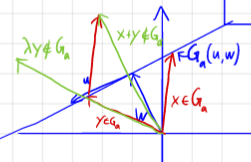
\includegraphics[width=.4\textwidth]{Dateien/00/11KeinUnterraum.PNG}
\end{tabular}
\end{Beispiel}
\begin{Beispiel}
{Ein weiterer Unterraum? (4/4)}
Ist $U:=\{\Matrix{x\\y\\z}\in\mathbb{R}^3\furdas z=x y, \,x,y\in\mathbb{R}\}$ ein Unterraum des $\mathbb{R}^3$?\\
Nein, denn $U$ ist nicht abgeschlossen bezüglich der Addition:\\
Seien $v:=\Matrix{1\\0\\0}$ und $w:=\Matrix{0\\1\\0}$ Vektoren aus $U$.\\
Die Summe $v+w=\Matrix{1\\1\\0}$ ist nicht aus $U$, da die dritte Komponente nicht mehr das Produkt aus den ersten beiden ist.\\
Ist $U$ abgeschlossen bezüglich der skalaren Multiplikation?
\end{Beispiel}
\begin{Def}
{Bezeichnungen verschiedener Funktionenräume}
Wir definieren für ein Intervall $I\subset \mathbb{R}$ verschiedene Klassen von Funktionen:\\
\begin{tabular}{l|l|l}
    \textbf{Bezeichnung} &\textbf{ Bedeutung }&\textbf{ Erklärung} \\
    \hline
    $\Abb(I,\mathbb{R})$ & $\{f:I\to\mathbb{R}\}$ & \parbox[t]{5.4cm}{Jegliche Funktionen von $I$ nach $\mathbb{R}$}\\
    $C(I,\mathbb{R})$ & $\{f:I\to\mathbb{R}\furdas f \text{ stetig}\}$ & \parbox[t]{5.4cm}{Stetige Funktionen von $I$ nach $\mathbb{R}$}\\
    $\Diff(I,\mathbb{R})$ & $\{f:I\to\mathbb{R}\furdas f \text{ diffbar}\}$ & \parbox[t]{5.4cm}{Differenzierbare Funktionen von $I$ nach $\mathbb{R}$}\\
    $C^k(I,\mathbb{R})$ & $\{f:I\to\mathbb{R}\furdas f\, k \text{-fach stetig diffbar}\}$ & \parbox[t]{5.4cm}{$k$-fach stetig differenzierbare\footnote{Das heißt, dass die $k$-te Ableitung stetig ist.} Funktionen von $I$ nach $\mathbb{R}$}
\end{tabular}
Jetzt wisst ihr also, was gemeint ist, wenn von $C^\infty$-Funktionen gesprochen wird.
\end{Def}
\begin{Satz}
{Satz}{Unterrauminklusion für Funktionenräume}
Für $1\leq k\in\mathbb{N}$ gilt die folgende Unterrauminklusion:
\begin{equation*}
    \mathbb{R}[x]_{\leq n}\subseteq C^\infty(I,\mathbb{R})\subseteq C^k(I,\mathbb{R})\subseteq\Diff(I,\mathbb{R})\subseteq C(I,\mathbb{R})\subseteq\Abb(I,\mathbb{R}).
\end{equation*}
Die Polynome sind also ein Unterraum der unendlich oft stetig differenzierbaren Funktionen, welche ein Unterraum der $k$-fach stetig differenzierbaren Funktionen sind, welche ein Unterraum der differenzierbaren Funktionen sind, welche ein Unterraum der stetigen Funktionen sind, welche wiederum ein Unterraum der Funktionen sind. Puh.
\end{Satz}

\subsubsection{Vokabelbombardement}
Es folgt nun eine Reihe von Definitionen, die alle eng miteinander verknüpft sind, also gut aufpassen! Die Beispiele sollen euch helfen, wenn ihr nicht direkt seht, was mit den Definitionen gemeint ist, ihr könnt sie aber auch erstmal überspringen, um euch einen Überblick zu verschaffen.\\
Im Folgenden sei $V$ stets ein Vektorraum über einem Körper $\mathbb{K}$ (z. B. über $\mathbb{R}$).
\begin{Def}
{Familien von Vektoren}
Eine \red{Familie}\footnote{Die Begriffe der Mathematiker sind z.T. direkt aus dem Leben gegriffen. Falls ihr irgendwann vorhabt, Topologie zu hören, wird euch vielleicht das \textit{Geschlecht} von Flächen über den Weg laufen, genauso wie man in der Funktionentheorie Funktionen ein Geschlecht zuweist. Auch die Begrifflichkeit \textit{fast alle} ist tatsächlich streng mathematisch definiert.} ist schlicht eine indizierte\footnote{jedem Element wird ein Index zugewiesen} Menge, z. B. $(v_i)_{i\in J}$ mit den Vektoren $v_i\in V$ und einer Indexmenge $J$.\\
Indexmengen dürfen bei Familien auch überabzählbar sein.
\end{Def}
Einen Spezialfall hatten wir mit den Folgen kennengelernt (z. B. $(a_n)_{n\in\mathbb{N}}$, $a_n\in\mathbb{R}$).\\
Hier waren die Elemente der Familie die reellen Zahlen $a_n$, die Indexmenge war $\mathbb{N}$.
\begin{Beispiel}
{Musterfamilie (1/2)}
Ein Beispiel aus $\mathbb{R}^3$ wäre die Familie $(v_i)_{i\in\{1,2,5\}}$ mit 
\begin{equation*}
    v_1:=\Matrix{1\\2\\3},\quad v_2:=\Matrix{1\\0\\0},\quad v_5:=\Matrix{2\\1\\0},
\end{equation*}
d. h. im Prinzip die Menge $\left\{\Matrix{1\\2\\3},\Matrix{1\\0\\0},\Matrix{2\\1\\0}\right\}$ mit indizierten Elementen.
\end{Beispiel}
\begin{Beispiel}
{Reelle Familie (2/2)}
Andererseits ist auch eine Familie mit reellem Index $a$ möglich:
\begin{equation*}
    (v_a)_{a\in\mathbb{R}}:=\BracedIn{\Matrix{a\\a^2\\-5a}}_{a\in\mathbb{R}}.
\end{equation*}
\end{Beispiel}
\begin{Def}
{Linearkombination}
Wenn wir einen Vektor $v\in V$ durch eine \underline{endliche} Familie von Vektoren $(v_i)_{i\in J}$, also $v_i=v_1,...,v_r$ mit Koeffizienten $\lambda_i$ aus $\mathbb{K}$ durch
\begin{equation*}
    \boxed{v=\sum_{i=1}^r\lambda_i v_i}
\end{equation*}
darstellen können, so nennen wir $v$ eine \red{Linearkombination} der Vektoren $(v_i)_{i\in J}$.
\end{Def}
\begin{Beispiel}[label=beisp:LinKombVektoren]
{Was ist möglich{,} was nicht?}
Wir betrachten die Vektoren
\begin{equation*}
    \boxed{v_1:=\Matrix{1\\2\\3},\quad v_2:=\Matrix{1\\1\\2},\quad v_3:=\Matrix{-1\\0\\-1},\quad v_4:=\Matrix{1\\4\\5}}.
\end{equation*}
$v_1$ kann als Linearkombination von $v_2$ und $v_3$ ausgedrückt werden, denn\\
$v_1=2v_2+v_3$.\\
$v_4$ kann nicht durch $v_1$ und $v_2$ dargestellt werden, denn das Gleichungssystem\\
$\lambda_1 v_1+\lambda_2 v_2=v_4$ ist nicht lösbar, wir wir hier sehen:
\begin{equation*}
    \Matrix{\lambda_1+\lambda_2\\2\lambda_1+\lambda_2\\3\lambda_2+2\lambda_2}=\Matrix{1\\4\\5}
\end{equation*}
Die erste Gleichung besagt $\lambda_1=1-\lambda_2$, woraus mit der zweiten\\$2\lambda_1+\lambda_2=4\Leftrightarrow 2-\lambda_2=4\Leftrightarrow\boxed{\lambda_2=2},\,\boxed{\lambda_1=-1}$ folgt.\\
Eingesetzt in die dritte ergibt dies aber $3\cdot2+2\cdot(-1)=5$. \Lightning
\end{Beispiel}
\begin{Def}
{Lineare Hülle}
Die Menge aller Vektoren aus $V$, die durch Linearkombination aus den Vektoren einer Familie $(v_i)_{i\in J}$ dargestellt werden können, nennt man \red{lineare Hülle}.\footnote{oder manchmal auch \red{lineares Erzeugnis}}\\
\textbf{Notation}:\\
$\Span{v_i}{i\in J}=\{v\furdas v\text{ ist Linearkombination der Familie } (v_i)_{i\in J}\}$.
\end{Def}
Anschaulich kann man sich dies vorstellen als der Unterraum, der durch die Vektoren der Familie aufgespannt wird - daher auch der Name.
\begin{Beispiel}{Vektoren aus der linearen Hülle}
Bezogen auf die Vektoren aus Beisp. \ref{beisp:LinKombVektoren} und unsere Feststellungen dort ist also
\begin{equation*}
    v_1\in\Spann{v_2,v_3}\text{ und }v_4\notin\Spann{v_1,v_2}
\end{equation*}
\end{Beispiel}
\begin{Def}
{Lineare Unabhängigkeit}
Eine besondere Bedeutung hat die Darstellung des Nullvektors als Linearkombination:\\
Wir nennen die Familie $(v_i)_{i\in J}$ \red{linear unabhängig}, wenn der Nullvektor nur durch Linearkombination der $(v_i)_{i\in J}$ dargestellt werden kann, wenn \underline{alle} Koeffizienten $\lambda_i=0$ sind, d. h.
\begin{equation*}
    \Vec{0}=\sum_{i=1}^r\lambda_iv_i\Rightarrow \lambda_i=0\,\forall i.
\end{equation*}
\end{Def}
Anders gesagt: Man kann keinen der Vektoren aus der Familie durch Linearkombination der anderen darstellen.
\begin{Beispiel}
{Vektoren des $\mathbb{R}^3$ (1/2)}
Sind die Vektoren $v_1$ und $v_2$ aus Beisp. \ref{beisp:LinKombVektoren} linear unabhängig?\\
Starte mit $\lambda_1v_1+\lambda_2v_2=0$, $\lambda_1, \lambda_2\in\mathbb{R}$.\\
Dann besagen die beiden ersten Zeilen der Gleichung
\begin{eqnarray*}
    (I)&&\,\lambda_1+\lambda_2=0\Rightarrow\lambda_1=-\lambda_2\\
    (II)&&\,2\lambda_1+\lambda_2=0\overset{(I)}{\Rightarrow}1(-\lambda_2)+\lambda_2=0\Rightarrow\lambda_2=0\Rightarrow\lambda_1=0
\end{eqnarray*}
Also sind $v_1$ und $v_2$ linear unabhängig.\\
Tatsächlich ist die Familie $(v_i)_{i\in\{1,2,3\}}$ linear abhängig und die Familie $(v_i)_{i\in\{1,2,4\}}$ linear unabhängig.
\end{Beispiel}
\begin{Beispiel}
{Monome (2/2)}
\Zz{Die Monome $(1,x,x^2,x^3,...,x^n)$ sind linear unabhängig im Vektorraum der Polynome $\mathbb{R}[x]{\leq n}$ von Grad $\leq n$.}
\Zb{Der Trick hier ist, dass die Gleichung $\sum_{k=0}^n\lambda_kx^k=0$ für alle $x\in\mathbb{R}$ erfüllt sein muss, also auch für $x=0$.\\
Für $x=0$ folgt sofort: $\lambda_0+\lambda_1\cdot0+0+...=0\Rightarrow\lambda_0\overset{!}{=}0$.\\
Der nächste Trick ist nun, einfach auf beiden Seiten der Gleichung abzuleiten, denn dann muss die Gleichung immer noch für alle $x\in\mathbb{R}$ erfüllt sein. Abgeleitet haben wir:
\begin{equation*}
    \sum_{k=1}^nk\lambda_kx^{k-1}=0\Leftrightarrow\sum_{k=0}^n(k+1)\lambda_{k+1}x^k=0\overset{x=0}{\Rightarrow}\lambda_1+2\lambda_2\cdot0+...=0\Rightarrow \lambda_1=0.
\end{equation*}
Wir argumentieren also wieder mit $x=0$.\\
Führen wir dies $n$ mal durch, erhalten wir $\lambda_i=0$ für alle $i\in\{0,1,...,n\}$.}
\end{Beispiel}
Die lineare Unabhängigkeit von Vektoren liefert uns eine schöne Eigenschaft:
\begin{Satz}
{Satz}{Eindeutigkeit der Darstellung durch linear unabhängige Familie}
Jeder Vektor $v$, der durch Linearkombination aus Vektoren einer linear unabhängigen Familie $(v_i)_{i\in J}$ dargestellt werden kann, d. h. $v\in\Span{v_i}{i\in J}$, besitzt eine \underline{eindeutige} Darstellung,
\begin{equation*}
    v=\sum_{i=1}^r\lambda_iv_i.
\end{equation*}
\end{Satz}
\begin{Def}
{Erzeugendensystem}
Wir nennen eine Familie $(v_i)_{i\in J}\in V$ ein \red{Erzeugendensystem}, wenn wir \underline{alle} Vektoren aus $V$ durch Linearkombination durch die $v_i$ darstellen können, d. h. $\Span{v_i}{i\in J}=V$.
\end{Def}
\begin{Def}
{Basis}
Ist ein Erzeugendensystem zudem linear unabhängig, so nennen wir es eine \red{Basis} von $V$.\\
Zusammen mit dem Satz über Eindeutigkeit hat also jeder Vektor $v\in V$ eine eindeutige Darstellung bezüglich einer Basis.
\end{Def}
\begin{Beispiel}
{Kanonische Basis (1/2)}
Die kanonische Basis des $\mathbb{R}^n$ ist $(e_1,e_2,...,e_n)$ mit $e_i:=(0,0,...,1,0,...)$.\footnote{mit der 1 an der $i$-ten Stelle}\\
Der Vektor $v=\Matrix{1\\-3.5}$ hab bzgl. der Standardbasis des $\mathbb{R}^2$ die Darstellung\\$v=1e_1-3.5e_2$.\\
Bezüglich einer anderen Basis wie z. B. $(b_1,b_2):=(e_1+e_2,e_1)$ ist die Darstellung jedoch\\
$v=-3.5b_1+2.5b_2$.
\end{Beispiel}
\begin{Beispiel}
{Monome als Basis (2/2)}
Die Monome $(1,x,x^2,...)$ bilden eine Basis der Polynome $\mathbb{R}[x]$.
\end{Beispiel}
\subsubsection{Aussagen über Basen}
Die folgenden Aussagen sind enorm wichtig für das Verständnis und sollten irgendwann auch intuitiv Sinn ergeben!
\begin{Satz}
{Satz}{Charakterisierung der Basis}
Eine Basis eines Vektorraumes $V$...
\begin{enumerate}
    \item ...ist stets ein \underline{minimales Erzeugendensystem}, d. h. jedes Erzeugendensystem von $V$ hat mindestens so viele Komponenten wie eine Basis.
    \item ...ist eine \underline{maximal linear unabhängige Familie}, d. h. es lässt sich kein weiterer Vektor hinzufügen, sodass die Familie linear unabhängig bleibt.
    \item Wie schon erwähnt: Jeder Vektor aus $V$ besitzt eine \underline{eindeutige} Darstellung bzgl. einer Basis.
    \item Jedes endliche Erzeugendensystem von $V$ enthält eine Basis (\red{Basisauswahlsatz}).
    \item Wenn $V$ eine endliche Basis besitzt,\footnote{d. h. die Basis besteht aus endlich vielen Vektoren} so ist jede Basis endlich und hat die \underline{gleiche Anzahl} an Elementen.
\end{enumerate}
\end{Satz}
\begin{Satz}
{Lemma}{Austauschlemma}
Wir dürfen den $k$-ten Basisvektor einer gegebenen Basis $(v_i)_{i\in J}\in V$ durch eine beliebige Linearkombination $w=\sum_{i=1}^n\lambda_iv_i$ austauschen, d. h. $(v_1,...,v_{k-1},w,v_{k+1},...)$ ist auch eine Basis, wenn $\lambda_k\neq 0$, wenn also $w$ einen endlichen Anteil von $v_k$ enthält.
\end{Satz}
\begin{Satz}
{Satz}{Steinitzscher Austauschsatz}
Wir können jede linear unabhängige Familie $(w_1,...,w_r)$ mithilfe einer Basis $(v_1,...,v_n)$ zu einer Basis von $V$ ergänzen.
\end{Satz}
\subsubsection{Dimension}
Vektorräume mit endlich vielen Basisvektoren können wir nun eindeutig über die Anzahl der Basisvektoren charakterisieren.
\begin{Def}
{Dimension}
Hat $V$ eine endliche Basis mit $n$ Elementen, so nennen wir diese Zahl die \red{Dimension} $\dim V=n$ von $V$.\\
Ist $V=\{\Vec{0}\}$, so ist $\dim V=0$. Andererseits ist $\dim V=\infty$.
\end{Def}
\begin{figure}[htbp]
\centering
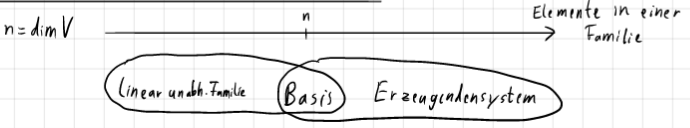
\includegraphics[width=.7\textwidth]{Dateien/00/11Dimensionschaubild.PNG}
\caption*{Veranschaulichung der Zusammenhänge zwischen linear unabhängiger Familie, Basis, Erzeugendensystem und Dimension.}
\end{figure}
\begin{Satz}
{Folgerung}{Zusammenfassung der Erkenntnisse}
Sei $V$ ein Vektorraum mit $\dim V= n$ und $(v_i)_{i\in J}$ eine Familie von Vektoren.
\begin{enumerate}
    \item Ist $(v_i)_{i\in J}$ \underline{linear unabhängig}, so hat sie \underline{höchstens} $n$ Elemente.
    \item Ist $(v_i)_{i\in J}$ \underline{linear unabhängig}, so ist sie genau dann eine Basis, wenn sie $n$ Elemente hat.
    \item Ist $(v_i)_{i\in J}$ ein \underline{Erzeugendensystem}, so hat sie \underline{mindestens} $n$ Elemente.
    \item Ist $(v_i)_{i\in J}$ ein \underline{Erzeugendensystem}, so ist sie genau dann eine Basis, wenn sie $n$ Elemente hat.
\end{enumerate}
\end{Satz}
\blue{Das waren jetzt sehr viele Definitionen und Sätze, die sich gegenseitig ergänzen. Nehmt euch auf jeden Fall die Zeit, alle Zusammenhänge zu verstehen!}
\subsection{Gaußscher Algorithmus}
\blue{Wir gucken uns nun einen sehr nützlichen Algorithmus an, um Basen eines Vektorraums aus einem Erzeugendensystem zu bestimmen.\\
Dieser hilft zudem bei der Überprüfung linearer Unabhängigkeit und beim Lösen linearer Gleichungssysteme.}
\begin{Satz}
{Merksatz}{Gaußscher Algorithmus}
Wir gehen bei einem Gleichungssystem oder bei gegebenen Vektoren, bei denen fraglich ist, ob sie eine Basis bilden, folgendermaßen vor (falls etwas unklar ist, siehe die folgenden Beispiele):
\begin{enumerate}
    \item Schreibe die Vektoren oder Koeffizienten als Matrix.
    \item
\begin{tabular}{c l}
\parbox[b]{9.5cm}{
Wende die folgenden erlaubten Umformungen an, um die Matrix auf \textit{Zeilenstufenform} zu bringen:
} & 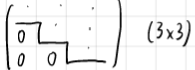
\includegraphics[width=.25\textwidth]{Dateien/00/11Zeilenstufenform.PNG}
\end{tabular} 
    \begin{enumerate}
        \item Vertauschen zweier Zeilen.
        \item Multiplizieren von Zeilen mit Skalaren $\lambda\in\mathbb{K}\setminus\{0\}$.
        \item Addieren von Vielfachen einer Zeile zu anderen Zeilen.
    \end{enumerate}
    \item Bei Gleichungungssystemen: Zurückführen auf die Gleichungen und diese von unten ausgehend zeilenweise abarbeiten.\\
    Beim Finden der Basis: Einfach die Nicht-Null-Zeilen ablesen.
\end{enumerate}
\end{Satz}
\begin{Beispiel}
{Lösen eines Gleichungssystems (1/4)}
Zu lösen seien die Gleichungen
\begin{align*}
    2x+3y+4z&=10\quad (I)\\
    6y-2z&=5\quad (II)\\
    -8x+z&=12\quad (III).
\end{align*}
\begin{enumerate}
    \item Wir schreiben die Koeffizienten als Matrix:
\begin{center}
    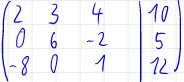
\includegraphics[width=.2\textwidth]{Dateien/00/11GaussA1.PNG}
\end{center}
    \item Wir wenden die erlaubten Umformungen an:
\begin{center}
    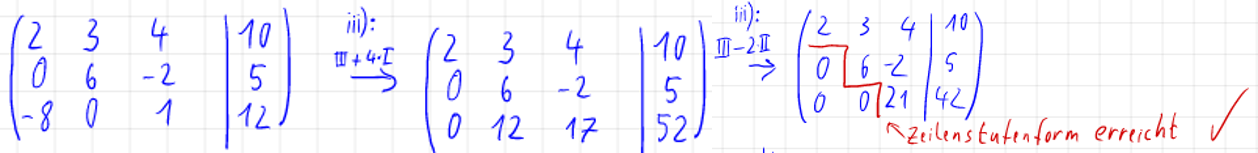
\includegraphics[width=.7\textwidth]{Dateien/00/11GaussA2.PNG}
\end{center}
    \item Wir führen dies auf die Gleichungen zurück und arbeiten uns von unten nach oben durch:
\begin{center}
    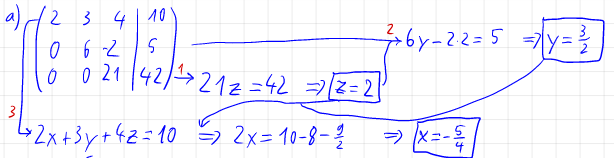
\includegraphics[width=.6\textwidth]{Dateien/00/11GaussA3.PNG}
\end{center}
\end{enumerate}
\begin{equation*}
    \Matrix{x\\y\\z}=\Matrix{-5/4\\3/2\\2}
\end{equation*}
löst also das Gleichungssystem.\\
\blue{\textbf{Anmerkung}:\\
Wir werden bald sehen, dass wir das Gleichungssystem auch so aufschreiben können:
\begin{center}
    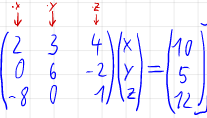
\includegraphics[width=.2\textwidth]{Dateien/00/11GaussA4.PNG}
\end{center}
}
\end{Beispiel}
\begin{Beispiel}
{Finden einer Basis (2/4)}
Wir suchen eine Basis des Unterraumes $U:=\Span{v_i}{i\in\{1,2,3\}}\subseteq\mathbb{R}^4$ mit den Vektoren
\begin{equation*}
    v_1=\Matrix{-2\\-2\\-5\\6},\quad v_2=\Matrix{1\\1\\2\\-2},\quad v_3=\Matrix{4\\4\\10\\-12}.
\end{equation*}
\begin{enumerate}
    \item Wir schreiben die Vektoren als Zeilen in eine Matrix:
\begin{center}
    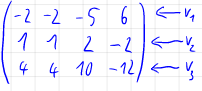
\includegraphics[width=.2\textwidth]{Dateien/00/11GaussB1.PNG}
\end{center}
    \item Wir wenden die erlaubten Umformungen an:
\begin{center}
    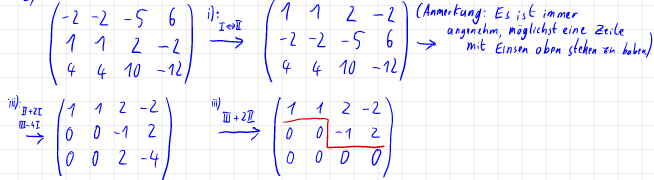
\includegraphics[width=.7\textwidth]{Dateien/00/11GaussB2.PNG}
\end{center}
    \item Wir führen dies auf Basisvektoren zurück
\begin{center}
    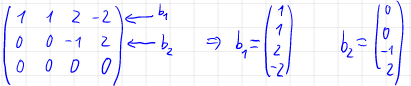
\includegraphics[width=.6\textwidth]{Dateien/00/11GaussB3.PNG}
\end{center}
\end{enumerate}
$U$ ist also ein zweidimensionaler Untervektorraum des $\mathbb{R}^4$.\\
\blue{\textbf{Anmerkung}:\\
Zwar ist diese Basis nicht eindeutig, aber die Anzahl der Basisvektoren ist durch die Dimension des Unterraums festgelegt.}
\end{Beispiel}
\begin{Beispiel}
{Lineare Unabhängigkeit und Basis prüfen (3/4)}
Bilden die folgenden Vektoren eine Basis des $\mathbb{R}^3$?
\begin{equation*}
    v_1=\Matrix{0\\1\\2},\quad v_2=\Matrix{2\\1\\0},\quad v_3=\Matrix{1\\0\\2}
\end{equation*}
Wenn sie linear unabhängig sind, ist das der Fall (da $\dim \mathbb{R}^3=3=\#v_i$).\\
Wir prüfen also, ob das lineare Gleichungssystem $\lambda_1v_1+\lambda_2v_2+\lambda_3v_3=\Vec{0}$ nur durch $\lambda_1=\lambda_2=\lambda_3=0$ zu lösen ist. Das können wir folgendermaßen aufschreiben:
\begin{center}
    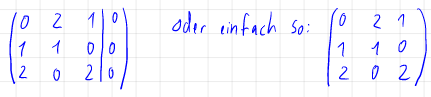
\includegraphics[width=.4\textwidth]{Dateien/00/11GaussC1.PNG}
\end{center}
Die zweite Schreibweise geht, da die rechte Seite der Gleichung (die Nullen) durch die Gauß-Operationen nicht geändert wird. Damit haben wir dann
\begin{center}
    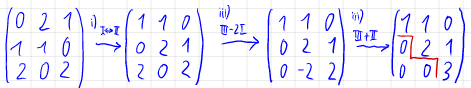
\includegraphics[width=.5\textwidth]{Dateien/00/11GaussC2.PNG}
\end{center}
Diese Gleichungen (also $3\lambda_3=0$, $2\lambda_2+\lambda_3=0$ und $\lambda_1+\lambda_2=0$) können tatsächlich nur durch $\lambda_1=\lambda_2=\lambda_3=0$ gelöst werden.\footnote{das kann man auch daran sehen, dass in der Zeilenstufenform keine Nullzeile mehr auftritt.}\\
Also ist die Familie $(v_i)_{i\in\{1,2,3\}}$ linear unabhängig.\\
Da die Anzahl der Elemente mit der Dimension 3 des $\mathbb{R}^3$ übereinstimmt, ist sie eine Basis des $\mathbb{R}^3$.
\end{Beispiel}
\begin{Beispiel}
{Lineare Unabhängigkeit und Basis prüfen (4/4)}
Bilden die folgenden Vektoren eine Basis des $\mathbb{R}^4$?
\begin{equation*}
    v_1=\Matrix{2\\-2\\6\\4},\quad v_2=\Matrix{1\\0\\2\\1},\quad v_3=\Matrix{2\\3\\0\\0},\quad v_4=\Matrix{1\\1\\1\\0}
\end{equation*}
Erneut: Gleichung für die lineare Abhängigkeit lösen:
\begin{equation*}
     \lambda_1v_1+\lambda_2v_2+\lambda_3v_3+\lambda_4v_4=\Vec{0}
\end{equation*}
\begin{center}
    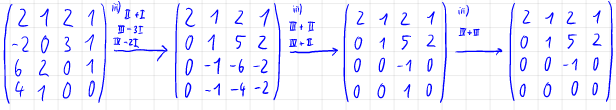
\includegraphics[width=.7\textwidth]{Dateien/00/11GaussD1.PNG}
\end{center}
Die letzte Gleichung lautet also $0\lambda_4=0$, d. h. wir können $\lambda_4$ beliebig wählen.\\
Wähle also $\lambda_4=:t\in\mathbb{R}\overset{(III)}{\Rightarrow}\boxed{\lambda_3=0}\overset{(II)}{\Rightarrow}\boxed{\lambda_2=-2t}\overset{(I)}{\Rightarrow}\boxed{\lambda_1=t/2}$.\\
Das Gleichungssystem wird also durch die Lösungsvektoren $L_t=t\Matrix{1/2\\-2\\0\\1}$ mit $t\in\mathbb{R}$ gelöst.\\
Betrachte als Beispiel $t=2:\quad v_1-4v_2+2v_4=\Vec{0}$ ist tatsächlich erfüllt.\\
Die Familie $(v_i)_{i\in\{1,2,3,4\}}$ ist also linear abhängig und kann daher kein Erzeugendensystem von $V$ sein.
\end{Beispiel}

\Tipps{1}{
\begin{enumerate}
    \item \begin{enumerate}
        \item Schaut euch die Definition der linearen Unabhängigkeit genau an - was folgt für die Koeffizienten von $\lambda_1v_1 +\lambda_2v_2=0$?
        \item Probiert verschiedene Beispiele aus, um ein Gefühl dafür zu bekommen.
    \end{enumerate}
    \item Denkt daran: Damit diese Funktionen linear unabhängig sind, müssen sie $\forall x\in \mathbb{R}$ linear unabhängig sein - vielleicht kann man daraus ja ein Gleichungssystem finden...\\
    Andererseits könnte es ja mit geschickten Koeffizienten ja auch klappen...
    \item Stumpfes Betrachten der Definition von linearen Abbildungen.
    \item
    \begin{enumerate}
        \item Hier müsst ihr einfach die Unterraumaxiome prüfen und schauen, was bei festem Grad schiefgehen könnte (etwa indem man durch Addition oder Multiplikation mit $\lambda\in\mathbb{R}$ außerhalb des Unterraums landet).
        \item Sollte schnell gemacht sein - evtl. hilft 3b).
        \item Hierfür einfach überlegen: Welche Polynome werden durch die zweite Ableitung auf den Nullvektor abgebildet? Diese bilden den Kern. Und: Auf welche Polynome wird ein Polynom von Grad $n$ durch die Abbildung abgebildet? Diese bilden das Bild. Gar nicht so schwierig, oder?
    \end{enumerate}
    \item \begin{enumerate}
        \item Schaut euch die Definition der inneren direkten Summe von Unterräumen an. Vielleicht ist der Durchschnitt ein guter Ansatz.
        \item Ein bisschen überlegen, wie nochmal die Dimension definiert war.
        \item Surjektivität bedeutet bei linearen Abbildungen $F:V\to W$, dass $\dim(\im(F))=\dim(W)$ ist.
        \item Injektivität bedeutet bei linearen Abbildungen, dass $\dim(\ker(F))=0$ ist, nur der Nullvektor aus $V$ wird also auf den Nullvektor aus $W$ abgebildet. Was ist hier aber der Nullvektor des Zielraumes?
    \end{enumerate}
\end{enumerate}}